\documentclass[oneside,10pt]{book}
\usepackage{graphicx}
\graphicspath{{pictures/}}% Specifies where pictures are stored
\usepackage{docmute} % for muting preamble of input files
\usepackage[top=0.65in,bottom=0.50in,left=0.75in,right=0.75in]{geometry}
\usepackage{amsmath}
\usepackage{amssymb}
\usepackage{multicol}
\usepackage{booktabs}
\usepackage[shortlabels]{enumitem}

\usepackage[activate={true,nocompatibility},final,tracking=true,kerning=true,spacing=true,factor=1100,stretch=10,shrink=10]{microtype}

\usepackage{subcaption} % for \captionof command
\usepackage{mathpazo} % Times
\usepackage[T1]{fontenc}
\usepackage[semibold]{raleway}

\usepackage[usenames,dvipsnames,svgnames]{xcolor} % for colors
\definecolor{ocre}{RGB}{0,135,255} % main color
\definecolor{maincolor}{RGB}{0,145,255} % main color
\definecolor{cqcqcq}{rgb}{0.75294117,0.75294117647,0.75294117647}

\usepackage{tikz}
\usetikzlibrary{arrows.meta, arrows}

\usepackage{xargs}
\usepackage{colortbl} % for colored tables
\usepackage{hyperref}
%\hypersetup{
    %colorlinks=true,
    %linkcolor=blue,
    %filecolor=magenta,
    %urlcolor=cyan,
%}





\makeatletter
%%%%%%%%%%%%%%%%%%%%%%%%%%%%%%%%%%%%%%%%%%%%%%%%%%%%%%%%%%%%%%%%%%%
% Set indent to zero, but save value just in case
%%%%%%%%%%%%%%%%%%%%%%%%%%%%%%%%%%%%%%%%%%%%%%%%%%%%%%%%%%%%%%%%%%%
\newlength\tindent
\setlength{\tindent}{\parindent}
\setlength{\parindent}{0pt}
\renewcommand{\indent}{\hspace*{\tindent}}
%%%%%%%%%%%%%%%%%%%%%%%%%%%%%%%%%%%%%%%%%%%%%%%%%%%%%%%%%%%%%%%%%%%
%%%%%%%%%%%%%%%%%%%%%%%%%%%%%%%%%%%%%%%%%%%%%%%%%%%%%%%%%%%%%%%%%%%

\newcounter{ExampleCounter}[section]
\newcommand{\example}{%
  \vspace{4pt minus 3pt}
  \par%
  \refstepcounter{ExampleCounter}%
  \noindent\textbf{Example~\arabic{ExampleCounter}.\,~}%
}



%%%%%%%%%%%%%%%%%%%%%%%%%%%%%%%%%%%%%%%%%%%%%%%%%%%%%%%%%%%%%%%%%%%
% grid command
%%%%%%%%%%%%%%%%%%%%%%%%%%%%%%%%%%%%%%%%%%%%%%%%%%%%%%%%%%%%%%%%%%%
\newcommand{\grid}[1]{%
\begin{tikzpicture}
  \draw[step=.5cm,cqcqcq,very thin] (-#1/2,-#1/2) grid (#1/2,#1/2);
\end{tikzpicture}
}


\newcommandx{\cart}[3][2=1,3={}]{%
\par
\begin{tikzpicture}[scale=#2]
  \draw[step=.5cm,cqcqcq,very thin] (-#1/2,-#1/2) grid (#1/2,#1/2);
  \draw[<->, black] (-#1/2,0) -- (#1/2,0);
  \draw[<->, black] (0, -#1/2) -- (0, #1/2);
  #3
\end{tikzpicture}
\par
}


\newcommandx{\cartX}[6][5=1,6={}]{%
\par
\begin{tikzpicture}[scale=#5]
  \draw[step=1cm,cqcqcq,very thin] (#1,#3) grid (#2,#4);
  \draw[<->, black] (#1,0) -- (#2,0);
  \draw[<->, black] (0, #3) -- (0, #4);
  #6
\end{tikzpicture}
\par
}
%%%%%%%%%%%%%%%%%%%%%%%%%%%%%%%%%%%%%%%%%%%%%%%%%%%%%%%%%%%%%%%%%%%
%%%%%%%%%%%%%%%%%%%%%%%%%%%%%%%%%%%%%%%%%%%%%%%%%%%%%%%%%%%%%%%%%%%


%%%%%%%%%%%%%%%%%%%%%%%%%%%%%%%%%%%%%%%%%%%%%%%%%%%%%%%%%%%%%%%%%%%%%%%%%%%
% Headings
%%%%%%%%%%%%%%%%%%%%%%%%%%%%%%%%%%%%%%%%%%%%%%%%%%%%%%%%%%%%%%%%%%%%%%%%%%%


\usepackage{titlesec}

\titleformat{\chapter}[display]
  {\sffamily\huge\bfseries}{\color{maincolor}
  {\chaptertitlename\ \thechapter}}{0pt}{\Huge}[]
\titleformat{\section}
  {\sffamily\LARGE\bfseries}
  {\color{maincolor}{\thesection}}{8pt}{}[]
\titleformat{\subsection}
  {\sffamily\Large\bfseries}{}{0ex}{}
\titleformat{\subsubsection}
  {\sffamily\normalsize\bfseries}{\thesubsubsection}{1ex}{}
\titleformat{\paragraph}[runin]
  {\sffamily\normalsize\bfseries}{\theparagraph}{1em}{}
\titleformat{\subparagraph}
  {\sffamily\LARGE\bfseries}
  {\color{maincolor}{\thesection}}{8pt}{}[]

\titlespacing*{\chapter} {0in}{0pt}{9pt}
\titlespacing*{\section} {0in}{3.5ex plus 1ex minus .2ex}{3.3ex plus .2ex}
\titlespacing*{\subsection} {0pt}{3.25ex plus 1ex minus .2ex}{1.5ex plus .2ex}
\titlespacing*{\subsubsection}{0pt}{3.25ex plus 1ex minus .2ex}{0.5ex plus .2ex}
\titlespacing*{\paragraph} {0pt}{3.25ex plus 1ex minus .2ex}{1em}
%\titlespacing*{\subparagraph} {\parindent}{3.25ex plus 1ex minus .2ex}{1em}
\titlespacing*{\subparagraph} {-0in}{3.5ex plus 1ex minus .2ex}{2.3ex plus .2ex}

\renewcommand{\bottomtitlespace}{2.5in}
%\newcommand{\sectionbreak}{\clearpage}
%\newcommand{\chapterbreak}{\cleardoublepage}


%%%%%%%%%%%%%%%%%%%%%%%%%%%%%%%%%%%%%%%%%%%%%%%%%%%%%%%%%%%%%%%%%%%%%%
%%%%%%%%%%%%%%%%%%%%%%%%%%%%%%%%%%%%%%%%%%%%%%%%%%%%%%%%%%%%%%%%%%%%%%

\newcommand{\setsection}[2]{%
  \setcounter{chapter}{#1}
  \setcounter{section}{#2}
  \addtocounter{section}{-1}

}

%%%%%%%%%%%%%%%%%%%%%%%%%%%%%%%%%%%%%%%%%%%%%%%%%%%%%%%%%%%%%%%%%%%%%%%%%%%
% Table of Contents Styling
%%%%%%%%%%%%%%%%%%%%%%%%%%%%%%%%%%%%%%%%%%%%%%%%%%%%%%%%%%%%%%%%%%%%%%%%%%%


\usepackage{titletoc} % Required for manipulating the table of contents
\contentsmargin{0cm} % Removes the default margin


% Part text styling
\titlecontents{part}[0cm]
{\addvspace{20pt}\centering\large\bfseries}
{}
{}
{}

% Chapter text styling
\titlecontents{chapter}[1.00cm] % Indentation
{\addvspace{5pt}\Large\sffamily\bfseries} % Spacing and font options for chapters
{\color{maincolor}\contentslabel[\Large\thecontentslabel]{1.00cm}\color{maincolor}} % Chapter number
{\color{maincolor}}
{\color{maincolor}\Large\;\titlerule*[.5pc]{.}\;\thecontentspage} % Page number

% Section text styling
\titlecontents{section}[1.75em] % Indentation
{\addvspace{5pt}\large\sffamily\bfseries} % Spacing and font options for chapters
{\color{maincolor}\contentslabel[\large\thecontentslabel]{1.75em}\color{black}} % Chapter number
{\color{black}}
{\color{black}\large\;\titlerule*[.5pc]{.}\;\thecontentspage} % Page number
[]

% Subsection text styling
\titlecontents{subsection}[1.75em] % Indentation
{\addvspace{0pt}\sffamily\small} % Spacing and font options for subsections
{} % Subsection number
{}
{\ \titlerule*[.5pc]{.}\;\thecontentspage} % Page number
[]


%%%%%%%%%%%%%%%%%%%%%%%%%%%%%%%%%%%%%%%%%%%%%%%%%%%%%%%%%%%%%%%%%%%%%%%%%%%
% PAGE HEADERS
%%%%%%%%%%%%%%%%%%%%%%%%%%%%%%%%%%%%%%%%%%%%%%%%%%%%%%%%%%%%%%%%%%%%%%%%%%%


\usepackage{ifthen}
\usepackage{fancyhdr} % Required for header and footer configuration

\pagestyle{fancy}

\renewcommand{\chaptermark}[1]{\markboth{\normalsize\bfseries\chaptername\ \thechapter\ \ #1}{}} % Chapter text font settings

\renewcommand{\sectionmark}[1]{\markright{\normalsize\thesection\hspace{5pt}#1}{}} % Section text font settings
\fancyhf{}


\fancyhead[R]{\sffamily\rightmark\hspace{5ex}\thepage}
%\fancyhead[L]{\ifthenelse{\isodd{\value{page}}}{}{\sffamily\thepage\hspace{5ex} \leftmark}}


\renewcommand{\headrulewidth}{0pt}
\renewcommand{\footrulewidth}{0pt} % Removes the rule in the footer

\addtolength{\headheight}{2.5pt} % Increase the spacing around the header slightly

%%%%%%%%%%%%%%%%%%%%%%%%%%%%%%%%%%%%%%%%%%%%%%%%%%%%%
%%%%%%%%%%%%%%%%%%%%%%%%%%%%%%%%%%%%%%%%%%%%%%%%%%%%%
% define a command to insert a blank page
        \newcommand{\insertblankpage}{%
          \newpage
          \thispagestyle{empty}
          \mbox{}
        \addtocounter{page}{-1}
          \newpage
        }
%%%%%%%%%%%%%%%%%%%%%%%%%%%%%%%%%%%%%%%%%%%%%%%%%%%%%
%%%%%%%%%%%%%%%%%%%%%%%%%%%%%%%%%%%%%%%%%%%%%%%%%%%%%



%%%%%%%%%%%%%%%%%%%%%%%%%%%%%%%%%%%%%%%%%%%%%%%%%%%%%
% Define Objectives Environment
%%%%%%%%%%%%%%%%%%%%%%%%%%%%%%%%%%%%%%%%%%%%%%%%%%%%%
\usepackage{environ}

\NewEnviron{objectives}[1]{%
\vspace{0.5em}
\noindent\textbf{\sffamily\Large Objectives}

\vspace{2mm}

\noindent%
#1

\vspace{-2.5mm}
\begin{multicols}{2}
\begin{itemize}[nosep,leftmargin=10.0pt]
    \BODY
\end{itemize}
\end{multicols}

}


%%%%%%%%%%%%%%%%%%%%%%%%%%%%%%%%%%%%%%%%%%%%%%%%%%%%%%%%%%%%%%%%%%%
% Create blue box for definitions and theorems
%%%%%%%%%%%%%%%%%%%%%%%%%%%%%%%%%%%%%%%%%%%%%%%%%%%%%%%%%%%%%%%%%%%


\tikzstyle{bluebox} = [fill=ocre!10, draw=ocre, very thick,
    rectangle, rounded corners, inner sep=10pt, inner ysep=5pt]
\tikzstyle{fancytitle} =[fill=ocre, text=white, rounded corners,
    inner ysep=3pt, inner xsep=5pt]



\def\blueboxstring{bluebox}


\newcommand{\bluebox}[2]{%
\par
\vspace{2mm minus 1mm}
\begin{tikzpicture}%
\node [bluebox] (box){%
    \begin{minipage}{0.99\textwidth}%
      \vspace{7pt}
      #2
    \end{minipage}
};
\node[fancytitle, right=10pt] at (box.north west) {%
  #1
};
\end{tikzpicture}
\par
\vspace{2mm}
}


%\NewEnviron{bluebox}[1]{%
%\par
%\vspace{2mm minus 1mm}
%\begin{tikzpicture}%
%\node [bluebox] (box){%
    %\begin{minipage}{0.99\textwidth}%
      %\vspace{7pt}
      %\expandafter\BODY
    %\end{minipage}
%};
%\node[fancytitle, right=10pt] at (box.north west) {%
  %#1
%};
%\end{tikzpicture}
%\par
%\vspace{2mm}
%}


%\let\blueboxenvironment\bluebox


%\def\bluebox#1{%
  %\ifx\@currenvir\blueboxstring%
    %\blueboxenvironment
  %\else
    %\blueboxcommand
  %\fi
%}



%%%%%%%%%%%%%%%%%%%%%%%%%%%%%%%%%%%%%%%%%%%%%%%%%%%%%
% Redefine vfill command to take optional parameter
%%%%%%%%%%%%%%%%%%%%%%%%%%%%%%%%%%%%%%%%%%%%%%%%%%%%%

\renewcommand{\vfill}[1][1]{\vspace{\stretch{#1}}}

\makeatother




\title{3.1 Lecture Notes}
\graphicspath{{3-1-lecture/}}

\AtBeginDocument{%
  \large
}

\begin{document}

\setsection{3}{1}

\section{Functions}

\textit{One of the most important concepts in all of mathematics is that of
  a function.} --T.P.~Dick and C.M.~Patton\\



\begin{objectives}{In this section, we will learn to}
  \item
    determine whether a relation is a function.
  \item
    use function notation.
  \item
    determine the domain of a function.
  \item
    determine the sum, difference, product, and quotient of two functions.
\end{objectives}


\bluebox{Definition -- Relation}{%
A \textbf{relation} in Mathematics is a correspondence between two sets.
}



\subsection{Maps and Ordered Pairs as Relations}
There are many different ways to represent relations.

\example
We can draw a correspondence between the set of states in the U.S. and a set
containing number of representatives for each state.

\begin{center}
  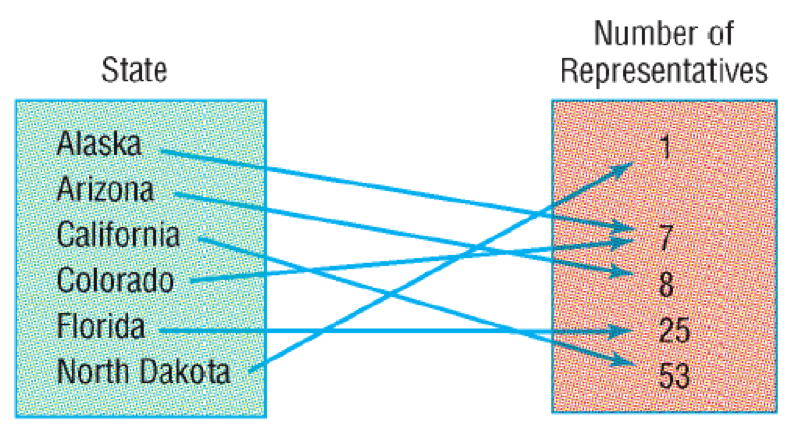
\includegraphics[scale=0.8]{Picture1.png}
\end{center}



This relation can also be expressed as a set of ordered pairs:\\
$\{
(\text{Alaska}, 7),
(\text{Arizona}, 8),
(\text{California}, 53),
(\text{Colorado}, 7),
(\text{Florida}, 25),
(\text{North Dakota}, 1)
\}$


\newpage


\bluebox{Definition -- Function}{%
  Suppose $A$ and $B$ are two non-empty sets.  A \textbf{function} from $A$ into
  $B$ is a relation that associates elements of $A$ with exactly one element of
  $B$.

}

\bluebox{Definition -- Domain and Range}{%
  %TODO: Write better definition of domain and range.
  From the previous definition, the set $A$ is known as the \textbf{domain} of the function.
  For each element $x$ in $A$, the corresponding element $y$ in $B$ is known as the
  \textbf{value} of the function at $x$ or the \textbf{image} of $x$.

  The set of all images of the elements of the domain is known as the
  \textbf{range} of the function.

}

\example
Which of these diagrams depicts a function?

{\centering
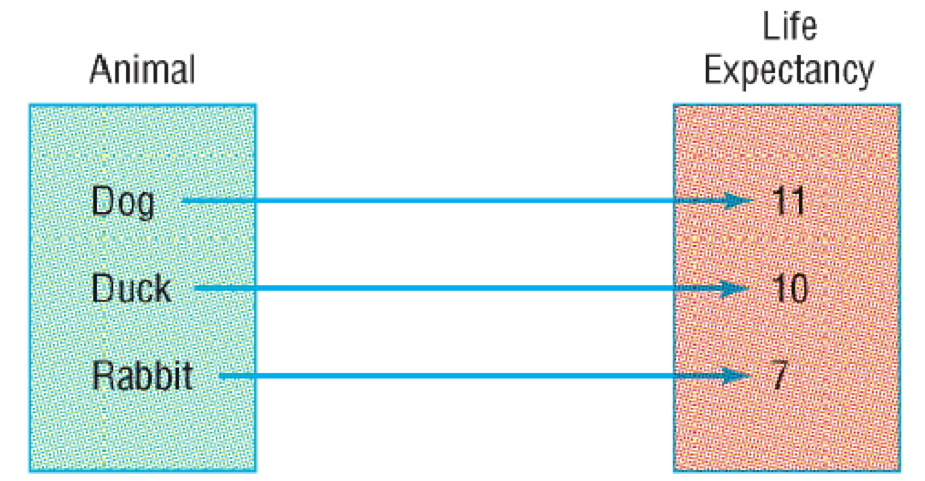
\includegraphics[scale=0.7]{Picture2.png}\\
\vspace{1cm}
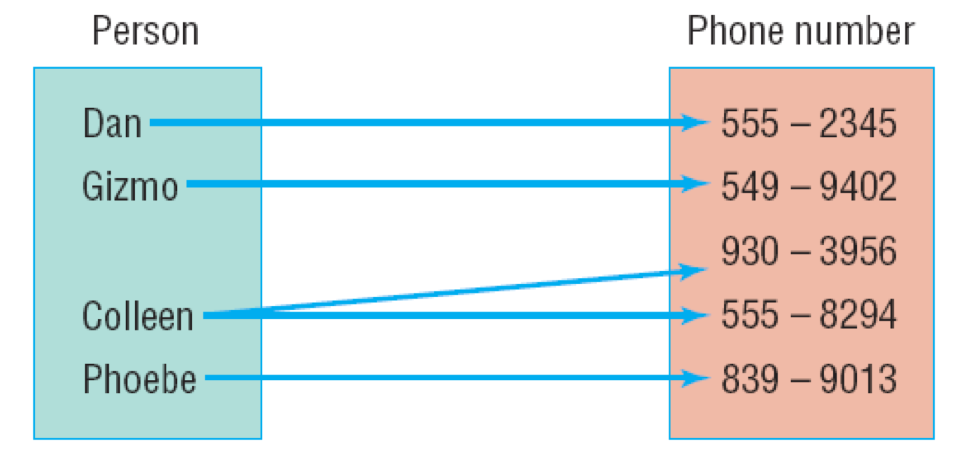
\includegraphics[scale=0.7]{Picture3.png}\\
}



\example
True or False. Each student's exam grade is a function of the student's IQ.
\vspace{1in}



\example
   Which of the following sets of ordered pairs describe a function?
  \begin{enumerate}[(a)]
    \item  $A = \{ (-2,1), (1,3), (1,4), (3,-1) \}$
    \item  $B = \{ (-2,1), (1,3), (2,3), (3,-1) \}$
  \end{enumerate}



\subsection{Relations Defined by Equations}

\example
Is $y=5x+1$ a function?
\vfill


\example
Is $y=x^2-1$ a function?
\vfill


\example
Is $|y|=x$ a function?
\vfill


\example
Is $x^2+y^2=1$ a function?
\vfill



\example
Is $y=x^3-x+1$ a function?
\vfill


\newpage


\subsection{Machine Interpretation of Functions}

\url{https://youtu.be/VUTXsPFx-qQ?t=213}

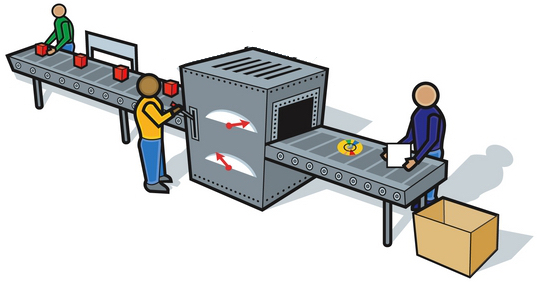
\includegraphics[width=0.5\linewidth]{3-1-lecture/001Production_Line.jpg}

Sometimes it is useful to think of functions as machines on an assembly line:
they take some input and produce some output. Like machines, functions have the
following characteristics:

\begin{enumerate}
  \item
    A function only accept certain things as inputs.
    That is, only numbers from the domain are allowed as inputs.
  \item
    A function is consistent.
    That is, for each input there is exactly one output.
\end{enumerate}



\subsection{Using Function Notation}

It is customary to use letters, such as $f$, to label functions.
We can think of a function $f$ as a process
by which each input $x$ is matched with only one output $y$.
Since the output is completely determined by the input $x$ and the process $f$, we symbolize the output with \textbf{function notation}: `$f(x)$', read `$f$ \textbf{of} $x$.'
In other words, $f(x)$ is the output which results by applying the process $f$ to the input $x$.
In this case, the parentheses here do not indicate multiplication, as they do elsewhere in Algebra.


\example
Suppose a function $g$ is described by applying the following steps,
in sequence
\begin{enumerate}
  \item  add 4
  \item  multiply by 3
\end{enumerate}
Determine $g(5)$ and find an expression for $g(x)$.
\vfill


\newpage


\example
Let $f(x) = x^2 +  4$.
Find and simplify the following.
\begin{enumerate}[(a)]
  \item $f(-1)$,\ $f(0)$,\, $f(2)$
  \item  $f(2x)$,\, $2 f(x)$
  \item $f(x+2)$,\, $f(x)+2$,\, $f(x) + f(2)$
\end{enumerate}
\vfill

\newpage


\subsection{Finding the Domain of a Function}


\example
Find the domain of each of the following functions.

\begin{enumerate}[(a)]
  \item
  $f(x) = x^2 + 5x $
  \vfill
  \item
    $g(x) = \dfrac{x-1}{x+4}$
  \vfill
  \item
    $h(x) = \sqrt{4 - 5x}$
  \vfill

\end{enumerate}


\subsection*{Check yourself!}


\begin{tabular}{@{}p{4.5in} c c c}
\textbf{Section Goals} & \textbf{Got It!} & \textbf{Getting It} & \textbf{Need Help}\\
I can identify which relation are functions. & $\square$ & $\square$ & $\square $ \\
I can identify the domain of a function that's been expressed as an equation. & $\square$ & $\square$ & $\square $ \\
I understand what an expression such as $f(3)$ means. & $\square$ & $\square$ & $\square $ \\
I know the difference between $f(2x)$ and $2f(x)$. & $\square$ & $\square$ & $\square $ \\


\end{tabular}





\end{document}
